\section{Part B.  Self Instructing Database:}
\label{part_b}
\subsection{Overview:}
Any standard database has considerable large number of configuration knobs. Databases needs to be tweaked with proper configuration for running efficiently with different workloads and hardware resources. Tweaking database configuration knowbs needs a great level of expertise from database administrator (DBA) because optimal configuration varies with the type of worloads. Beside that even finding optimal knob configurations might involve trial and error process for a DBA (which restrits the search spaces for knobs). An auto-configuring database system or self intructing database is a desirable feature to demand from database companies.


Human database administrators rely on experience and intuition to configure it. DRL process mimick same learning strategies i.e. learn from mistakes and correctness to maximize future rewards. Keeping this in mind we can explore how DRL can provide a solution automatic database tuning.


\subsection{Problem Formulation:}
Given a workload $\mathcal{W}$ with a knobs setting $\mathcal{C} = \{c_1,c_2,\ldots,c_{|\mathcal{C}|}\}$ a typical database outputs a log of metrics $\mathcal{M} = \{m_1,m_2,m_3,\ldots,m_{|\mathcal{M}|}\}$ as shown in Figure \ref{fig:database_01}.
The database keeps receiving workloads at some discrete interval of time and it runs with some configuration and outputs a metric log, which is also called a discrete time stochastic control process.

\begin{figure}[h]
	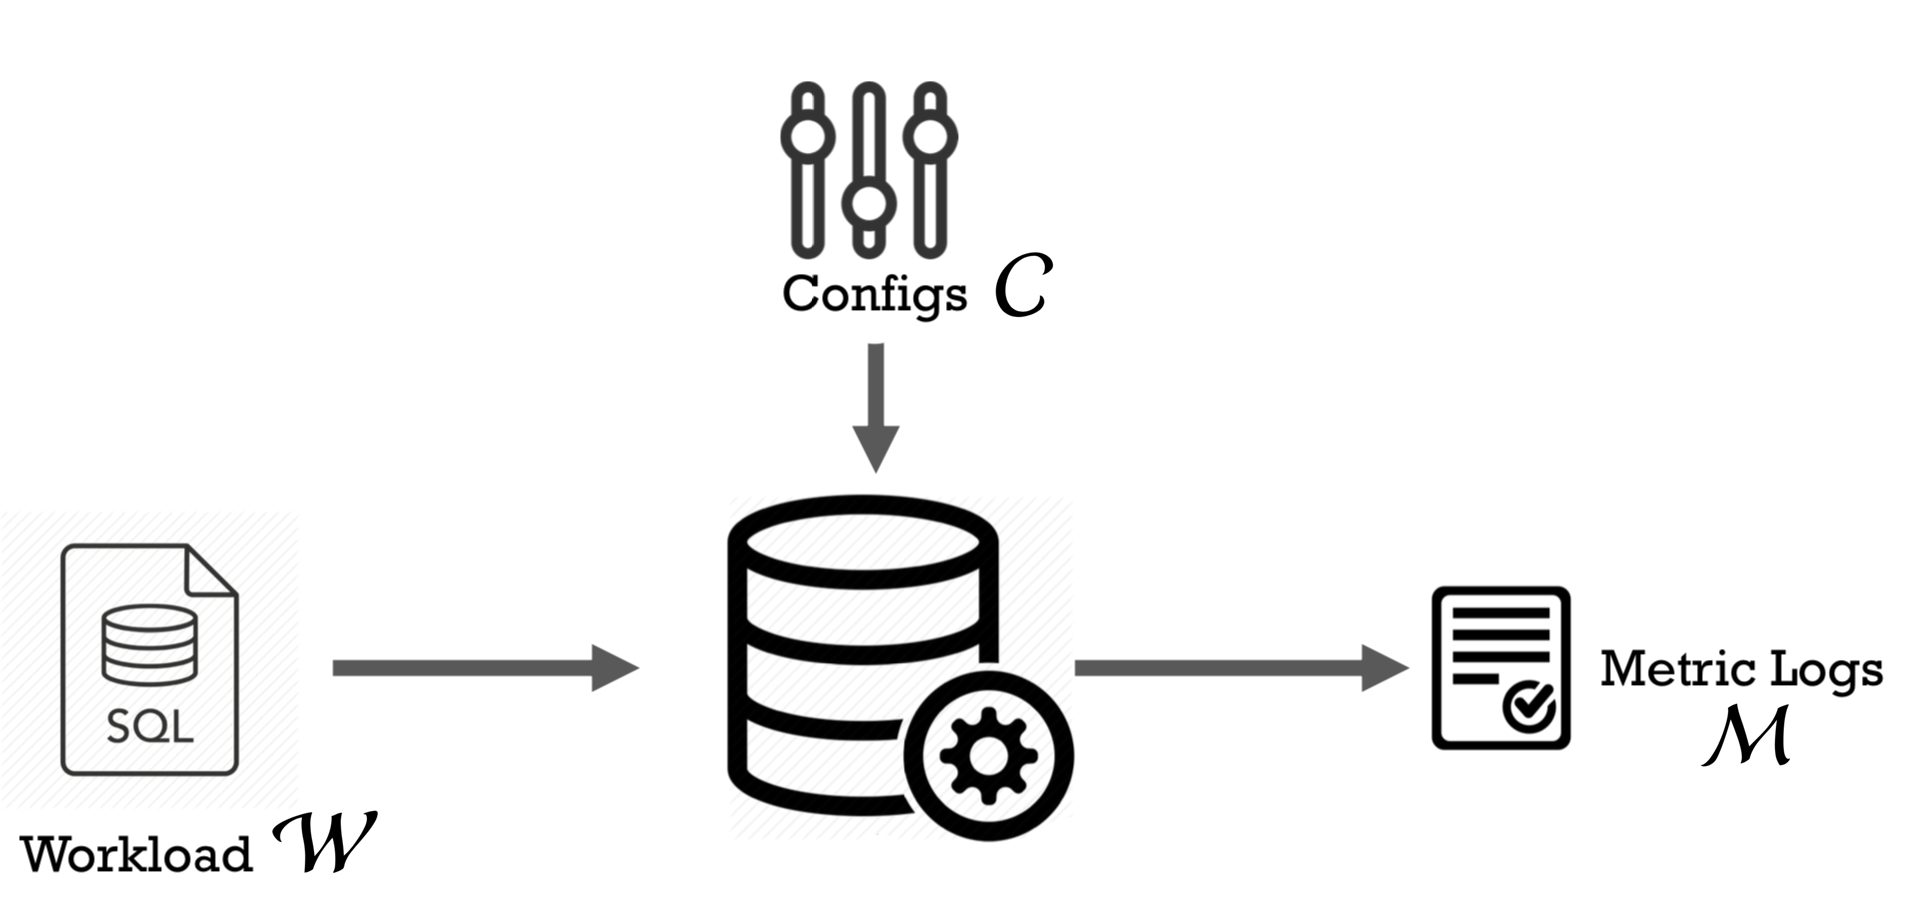
\includegraphics[width=0.9\linewidth ]{fig/database_01.png}
    \vspace{-2mm}
    \caption{A typical database system.}
    \label{fig:database_01}
\end{figure}


We can apply deep reinforcement learning to train a neural network in taking
over the database tuning process by optimizing configuration for observable database workload.
Essentially, we have to define a so called problem environment
consisting of the four following components to perform the learning as shown in Figure \ref{fig:database_agent}:


\textbf{1) Observable State:} This is also input to the neural network. This is typically the current workload in form of
query characteristics, for which the system should be optimised as well as the current state
of the configuration. Figure \ref{fig:database_agent} illustrates workload $\mathcal{W}_t$ is mapped to observation/state $\omega_t$ or $s_t$ for time stamp $t$.\\
\textit(Note: These notations are defined in Section \ref{formal_rl}).

\textbf{2) Actions:} An action is a bounded set of configuration $\mathcal{C}_t$ where each knobs can have a range of permissible values.
Changing the size of a database buffer is an example of action. Now we can represent $\mathcal{C}_t  \rightarrow a_t$.

\textbf{3) Reward:}
We map the metric $\mathcal{M}_t$ to rewards $r_t$. Since reward is a scalar function and metric $\mathcal{M}_t$ is a set of values representing the goodness and badness of database execution on workload $\mathcal{W}_t$.

\textbf{3) Hyperpaaramters for Neural Network:}
This includes properties of
the neural network (e.g. number of hidden layers, number of nodes per layer) as well as
properties of the learning process like the number of iterations.


We apply this process into a RL agent-database environment interaction process as shown in Figure \ref{fig:database_agent}.
In this process, at each time step $t$ we map metric $\mathcal{M}_t$ to rewards $r_t$. Similarly, workload $\mathcal{W}_t$ is mapped to observation/state $\omega_t$ or $s_t$, and configuration $C_t$ is mapped to action $a_t$.



\begin{figure}[t]
	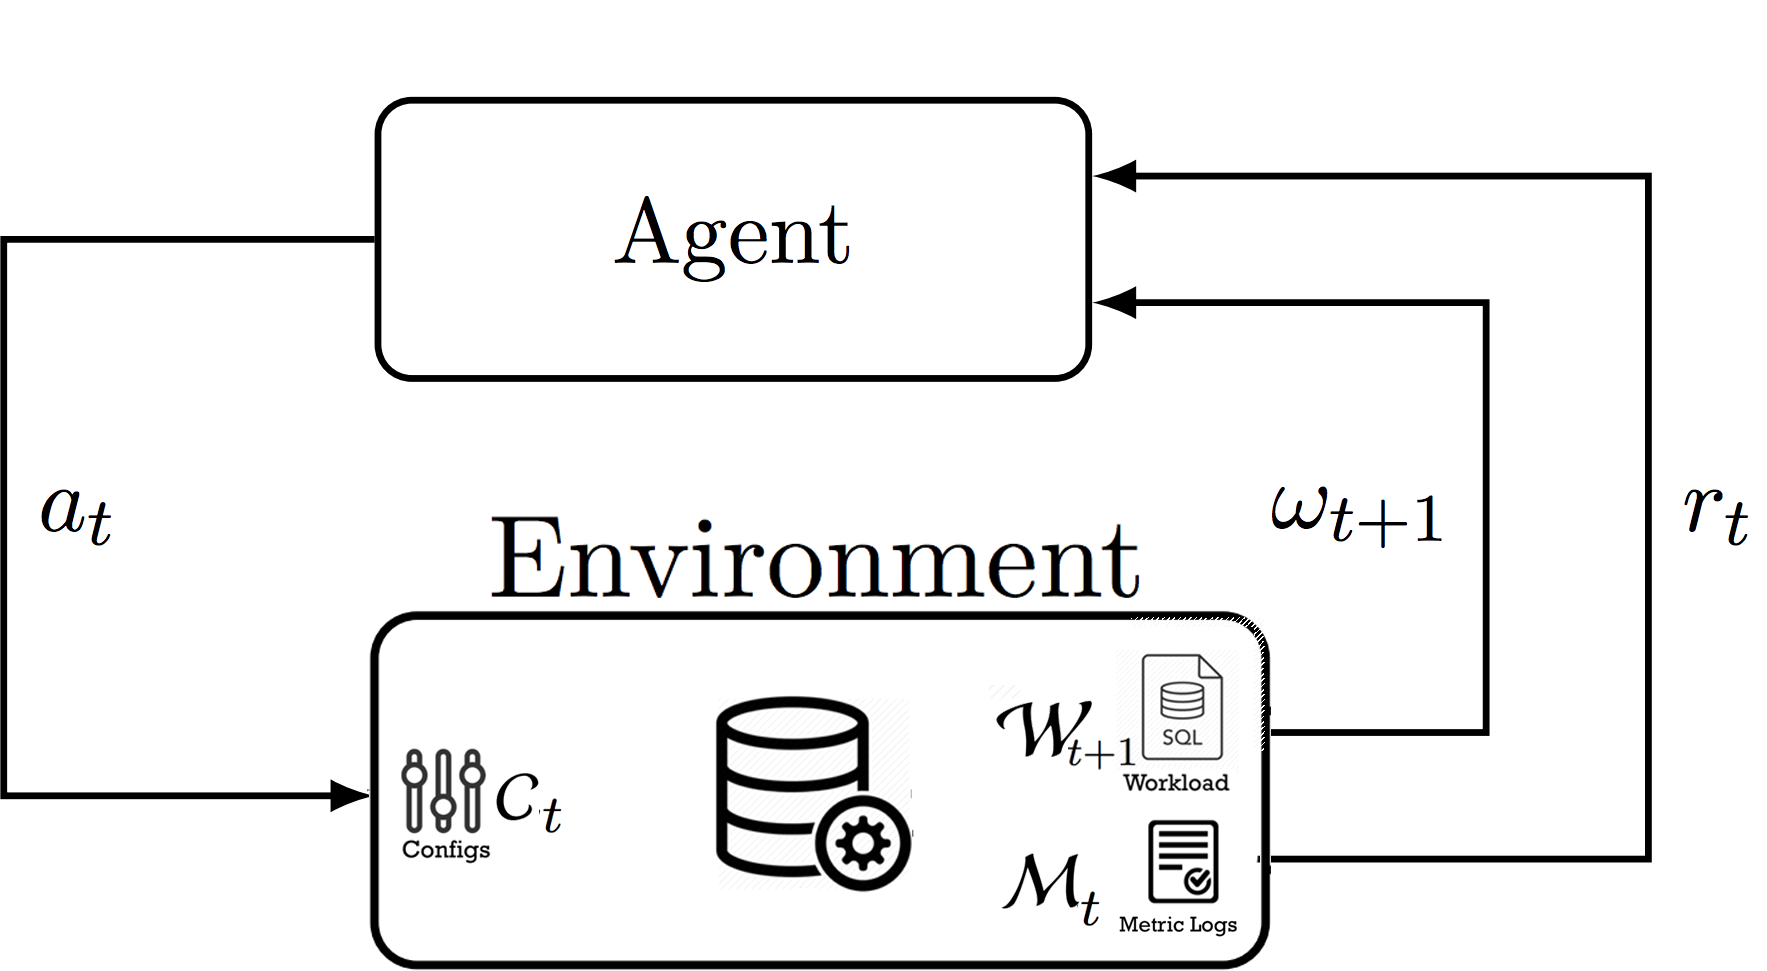
\includegraphics[width=0.9\linewidth ]{fig/database_agent.png}
    \vspace{-2mm}
    \caption{RL Agent-Database Environment Interaction.}
    \label{fig:database_agent}
\end{figure}


\subsection*{Multi-agent Deep RL:}







%%% Local Variables:
%%% mode: latex
%%% TeX-master: "main"
%%% End:
